\pdfinfoomitdate=1
\pdftrailerid{}
\pdfsuppressptexinfo=-1
\documentclass[border=6pt]{standalone}
\usepackage{amsmath,amssymb}
\usepackage{tikz}
\usetikzlibrary{arrows.meta,decorations.pathreplacing,positioning}
\begin{document}
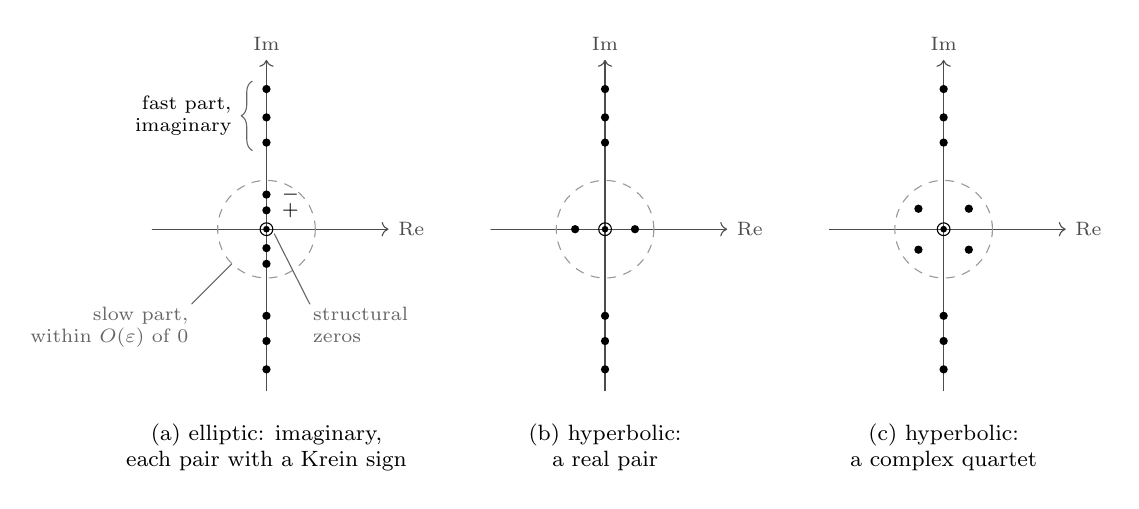
\begin{tikzpicture}[line cap=round, line join=round]
\draw[->, black!70] (-1.45,0) -- (1.55,0) node[right, font=\scriptsize] {Re};
\draw[->, black!70] (0.00,-2.05) -- (0.00,2.15) node[above, font=\scriptsize] {Im};
\draw[black!40, dashed] (0.00,0) circle (0.62);
\fill (0.00,1.10) circle (1.5pt);
\fill (0.00,1.42) circle (1.5pt);
\fill (0.00,1.78) circle (1.5pt);
\fill (0.00,-1.10) circle (1.5pt);
\fill (0.00,-1.42) circle (1.5pt);
\fill (0.00,-1.78) circle (1.5pt);
\draw (0.00,0) circle (2.3pt); \fill (0.00,0) circle (1.2pt);
\fill (0,0.24) circle (1.5pt); \fill (0,-0.24) circle (1.5pt);
\fill (0,0.44) circle (1.5pt); \fill (0,-0.44) circle (1.5pt);
\node[font=\scriptsize, anchor=west] at (0.07,0.24) {$+$};
\node[font=\scriptsize, anchor=west] at (0.07,0.44) {$-$};
\node[font=\footnotesize, align=center, anchor=north] at (0.00,-2.35) {(a) elliptic: imaginary,\\ each pair with a Krein sign};
\draw[->, black!70] (2.85,0) -- (5.85,0) node[right, font=\scriptsize] {Re};
\draw[->, black!70] (4.30,-2.05) -- (4.30,2.15) node[above, font=\scriptsize] {Im};
\draw[black!40, dashed] (4.30,0) circle (0.62);
\fill (4.30,1.10) circle (1.5pt);
\fill (4.30,1.42) circle (1.5pt);
\fill (4.30,1.78) circle (1.5pt);
\fill (4.30,-1.10) circle (1.5pt);
\fill (4.30,-1.42) circle (1.5pt);
\fill (4.30,-1.78) circle (1.5pt);
\draw (4.30,0) circle (2.3pt); \fill (4.30,0) circle (1.2pt);
\fill (3.92,0) circle (1.5pt); \fill (4.68,0) circle (1.5pt);
\node[font=\footnotesize, align=center, anchor=north] at (4.30,-2.35) {(b) hyperbolic:\\ a real pair};
\draw[->, black!70] (7.15,0) -- (10.15,0) node[right, font=\scriptsize] {Re};
\draw[->, black!70] (8.60,-2.05) -- (8.60,2.15) node[above, font=\scriptsize] {Im};
\draw[black!40, dashed] (8.60,0) circle (0.62);
\fill (8.60,1.10) circle (1.5pt);
\fill (8.60,1.42) circle (1.5pt);
\fill (8.60,1.78) circle (1.5pt);
\fill (8.60,-1.10) circle (1.5pt);
\fill (8.60,-1.42) circle (1.5pt);
\fill (8.60,-1.78) circle (1.5pt);
\draw (8.60,0) circle (2.3pt); \fill (8.60,0) circle (1.2pt);
\fill (8.28,0.26) circle (1.5pt); \fill (8.92,0.26) circle (1.5pt);
\fill (8.28,-0.26) circle (1.5pt); \fill (8.92,-0.26) circle (1.5pt);
\node[font=\footnotesize, align=center, anchor=north] at (8.60,-2.35) {(c) hyperbolic:\\ a complex quartet};
\draw[decorate, decoration={brace, amplitude=4pt}, black!60] (-0.18,1.00) -- (-0.18,1.88);
\node[font=\scriptsize, anchor=east, align=right] at (-0.32,1.44) {fast part,\\ imaginary};
\draw[black!60] (-0.44,-0.44) -- (-0.95,-0.95) node[anchor=north east, font=\scriptsize, align=right, inner sep=1pt] {slow part,\\ within $O(\varepsilon)$ of 0};
\draw[black!60] (0.10,-0.06) -- (0.55,-0.95) node[anchor=north west, font=\scriptsize, align=left, inner sep=1pt] {structural\\ zeros};
\end{tikzpicture}
\end{document}
